\chapter{Sistemas embebidos}
\label{conceptos}

En este capítulo se abordan conceptos relacionados al tipo de sistemas con los que se trabaja en el ámbito de la robótica. Entre ellos se encuentran algunas definiciones como la de \textit{Sistemas embebidos}, microcontroladores, interrupciones y ciertos comportamientos comunes de este tipo de sistemas.


\section{Definición}
Distintos autores proponen diferentes definiciones de sistemas embebidos:
\\\\
\noindent
``\textit{Un sistema computarizado dedicado a realizar un conjunto específico de funciones del mundo real, en lugar de proporcionar un entorno de computación generalizado.}''~\cite{douglass}
\\\\
\noindent
``\textit{Un sistema embebido es un sistema computarizado diseñado específicamente para su aplicación.}'' Debido a que su misión es más limitada que la de una computadora de propósito general, un sistema embebido tiene menos soporte para aspectos no relacionados con la ejecución de la aplicación.~\cite{elecia}
\\\\
\noindent
``\textit{Un sistema embebido es un sistema informático aplicado, a diferencia de otros tipos de sistemas informáticos como las computadoras personales (PCs) o las supercomputadoras.}''~\cite{noergaard2005embedded}
\\\\
\noindent		
El último autor comenta que los sistemas embebidos cumplen las siguientes afirmaciones:
\begin{itemize}
	\item Los sistemas embebidos son más limitados en funcionalidad de hardware y/o software que una computadora personal.
	\item Un sistema embebido está diseñado para realizar una función dedicada.
	\item Un sistema embebido es un sistema informático con requisitos de mayor calidad y fiabilidad que otros tipos de sistemas informáticos.
	\item Algunos dispositivos que se denominan sistemas embebidos, como los Asistentes Digitales Personales (\gls{pda}).
\end{itemize}

De las definiciones se puede concluir que un sistema embebido es una pieza clave que permite que hardware especializado cumpla con su propósito específico. A diferencia de los sistemas de propósito general, el software en un sistema embebido está diseñado para interactuar estrechamente con los componentes de hardware, respondiendo en tiempo real a eventos del entorno, ya sea para controlar actuadores, monitorear sensores o gestionar comunicaciones. Este software está optimizado para requisitos específicos como velocidad, consumo energético, y confiabilidad, lo que lo hace esencial en aplicaciones críticas como dispositivos médicos, sistemas automotrices y controles industriales.
	
En resumen, el software de un sistema embebido actúa como el cerebro que dirige y coordina los recursos del hardware para realizar funciones concretas. En la Tabla~\ref{tab:ejSistEmbebidos} extraída de \cite{noergaard2005embedded} encontramos ejemplos de dispositivos en los que se utilizan sistemas embebidos.

\begin{table}[h]
\caption{Ejemplos sistemas embebidos.}
    \centering
    \label{tab:ejSistEmbebidos}
    \begin{tabular}{|l|l|}
        \hline
        \textbf{Mercado} & \textbf{Dispositivo Embebido} \\ \hline
        Automotriz & Sistema de encendido \\ 
        & Control del motor \\ 
        & Sistema de frenos (Sistema Antibloqueo de Frenos - ABS) \\ \hline
        Electrónica de consumo & Decodificadores (DVDs, VCRs, Cajas de cable, etc.) \\ 
        & Asistentes Personales Digitales (\gls{pda}) \\ 
        & Electrodomésticos (Refrigeradores, Tostadoras, Microondas) \\ 
        & Automóviles \\ 
        & Juguetes/Juegos \\ 
        & Teléfonos/Celulares/Bípers \\ 
        & Cámaras \\ 
        & Sistemas de Posicionamiento Global (GPS) \\ \hline
        Control Industrial & Sistemas de control y robótica (Manufactura) \\ \hline
        Médico & Bombas de infusión \\ 
        & Máquinas de diálisis \\ 
        & Prótesis \\ 
        & Monitores cardíacos \\ \hline
        Redes & Routers \\ 
        & Hubs \\ 
        & Puertas de enlace \\ \hline
        Automatización de Oficina & Máquinas de fax \\ 
        & Fotocopiadoras \\ 
        & Impresoras \\ 
        & Monitores \\ 
        & Escáneres \\ \hline
    \end{tabular}
\end{table}

Otros autores \cite{lee2017introduction} describen sistemas \textit{ciber-físicos} (\Ac{CSP}\footnote{por sus siglas en inglés (cyber-physical system)}) como la integración de la computación con procesos físicos. Esta integración usualmente se lleva a cabo utilizando sistemas embebidos con ciclos de retroalimentación; en los cuales la parte computacional afecta al ámbito físico y viceversa. Los componentes que permiten la comunicación entre ambos mundos son sensores y actuadores.
Además, si tomamos en cuenta los ejemplos que se presentan tanto en \cite{noergaard2005embedded} como en \cite{lee2017introduction}, podemos decir que la mayoría de los sistemas embebidos realizan tareas de \textbf{control} sobre el mundo físico.

Con respecto al hardware en donde corren los sistemas embebidos podemos descatar que suele consistir en una placa o chip compacto que incluye:
\begin{itemize}
    \item \textbf{Unidad de Microcontrolador (MCU):} Un microcontrolador que integra un procesador, memoria y perif\'ericos en un solo chip. Es el componente principal que ejecuta el software.
    \item \textbf{Memoria Flash:} Utilizada para almacenar el programa y los datos no vol\'atiles.
    \item \textbf{Memoria RAM:} Proporciona almacenamiento temporal para datos en tiempo de ejecuci\'on.
    \item \textbf{Interfaces de entrada/salida:} Puertos \gls{GPIO}, \gls{ADC}, \gls{PWM} y otros para interactuar con sensores, actuadores y otros dispositivos externos.
    \item \textbf{Fuente de Energ\'ia:} Puede provenir de bater\'ias, adaptadores de corriente o incluso energ\'ia recolectada del entorno.
\end{itemize}
El tama\~no compacto y la integraci\'on de componentes distinguen a los sistemas embebidos de otros sistemas m\'as grandes como las computadoras de escritorio o los servidores. Se diferencian, además, en su poder de cómputo limitado tanto por el hardware (baja disponibilidad de memoria RAM, \gls{clock} de la CPU bajo, etc) como por la disponibilidad de energía eléctrica.

Existen varios microcontroladores multipropósito de uso comercial, tales como los producidos por la empresa Arduino \cite{arduinoMicro} o los similares de la familia  Raspberry Pi \cite{raspMicro}. La presentación de los mismos suele ser en forma de una placa preparada para conectar los inputs y outputs, como las que se observan en Figuras \ref{arduinoUNO} y \ref{raspberry}.

Por defecto, el microcontrolador ejecuta el software almacenado en su unidad flash, la cual debe ser grabada cada vez que se actualice el código. Dado esto y las limitaciones de hardware ya mencionadas, se deben tener ciertas consideraciones a la hora de escribir el código. En particular, se debe prestar atención a la performance del sistema, a la cantidad de librerías a utilizar, al uso de memoria RAM, etc.

\begin{figure}[h!]
	\caption{Arduino UNO}
	\label{arduinoUNO}
	\centering
    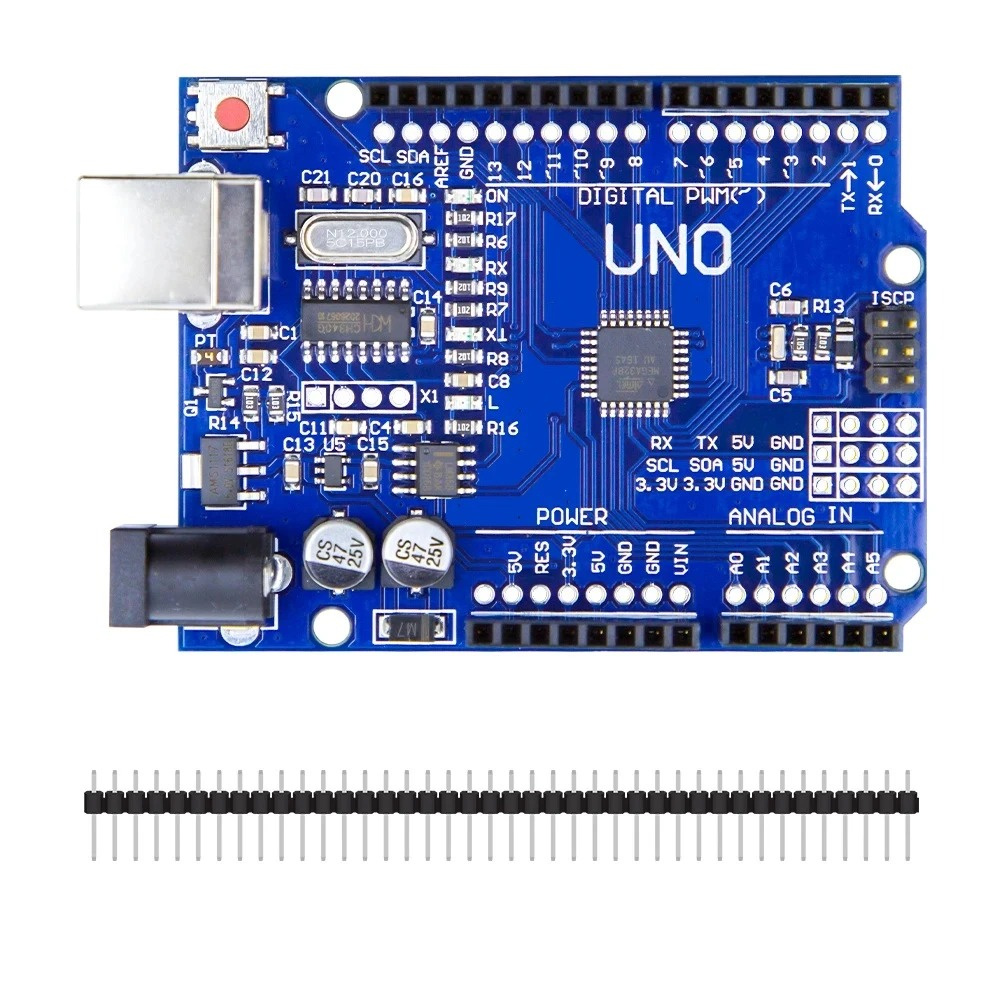
\includegraphics[width=0.5\linewidth]{arduinoUNO.jpeg}
\end{figure}


\begin{figure}[h!]
	\caption{Raspberry Pico 2}
	\label{raspberry}
	\centering
    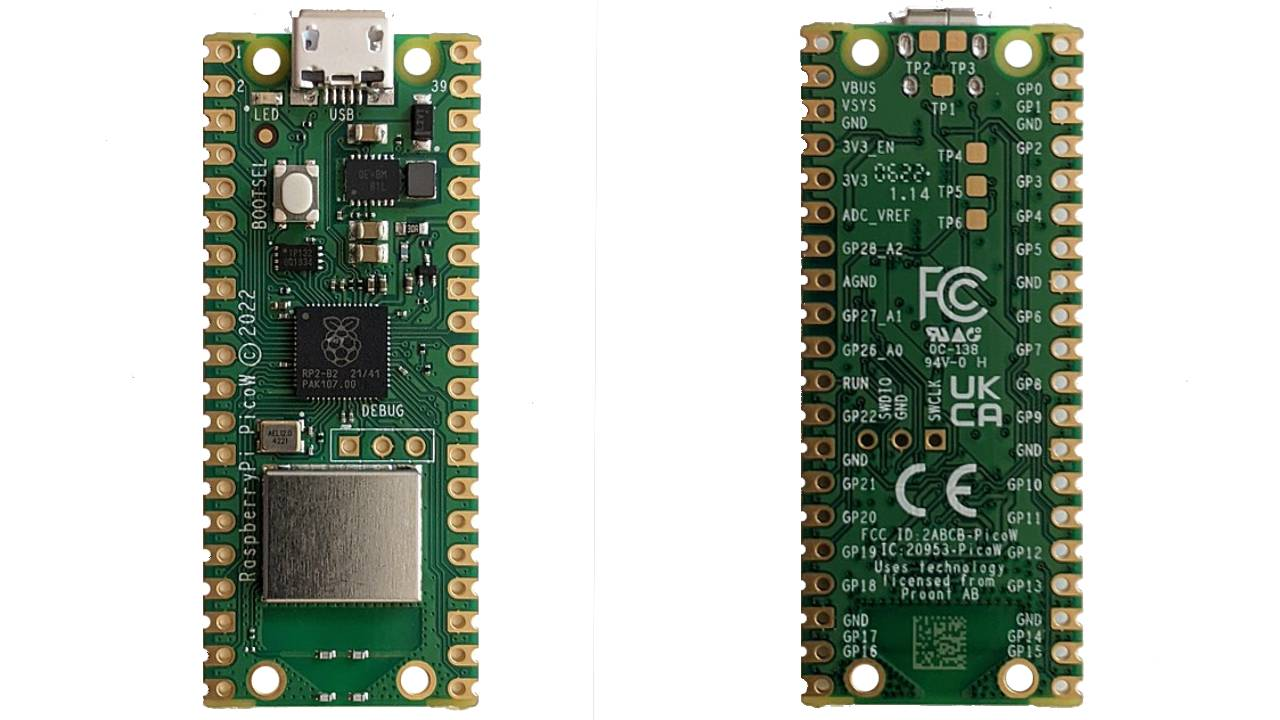
\includegraphics[width=0.6\linewidth]{raspberry_pico2.jpg}
\end{figure}


\section{Interrupciones}
\label{secInterrupciones}
Como se mencionó, el dispositivo en el que el software corre suele ser un microcontrolador (\gls{MCU}). Estos dispositivos poseen ciertas características particulares que los hacen ideales para trabajar en entornos cercanos al mundo real; entre ellas las interrupciones. Las mismas son un mecanismo de eventos que pausan la ejecución del programa principal para atender una tarea urgente. Funcionan como un mecanismo de respuesta automática que permite que el microcontrolador responda inmediatamente a eventos externos o internos sin depender de que el programa principal revise continuamente el estado de los dispositivos o variables asociadas a la generación de la interrupción.

Cuando ocurre una interrupción (por ejemplo, un cambio en un sensor o una solicitud de un actuador), el \gls{MCU} detiene su ejecución actual y salta a una rutina de servicio de interrupción (ISR, Interrupt Service Routine). Esta rutina es un fragmento de código predefinido que realiza las tareas necesarias, como leer un sensor o activar un actuador. Una vez finalizada la ejecución de la ISR, el \gls{MCU} retorna automáticamente al punto en el que se había interrumpido, reanudando el programa principal sin perder el flujo de ejecución. Siguiendo la Figura \ref{interrupt}, el \gls{MCU} se encuentra ejecutando el código principal cuando se produce una interrupción. En ese momento, detiene temporalmente dicha ejecución para atender la rutina de interrupción. Al completarse esta, el \gls{MCU} continúa la ejecución del código principal desde la primera instrucción que no había sido ejecutada, en este caso, la \textit{instrucción 3}.

\begin{figure}[H]
	\centering
    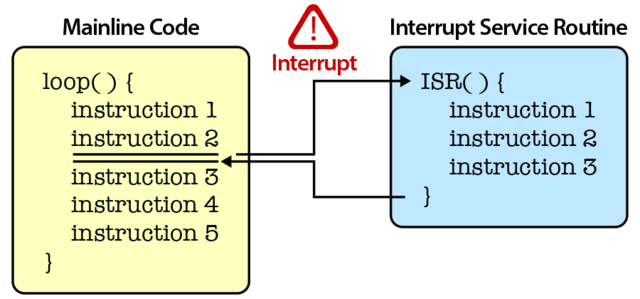
\includegraphics[width=0.7\linewidth]{components_interrupt.png}
    \caption{Diagrama interrupción extraído de \cite{imgInterrupciones}.}
    \label{interrupt}
\end{figure}

Este mecanismo es esencial en sistemas embebidos, especialmente en aquellos que controlan sensores y actuadores, porque permite un control eficiente de múltiples dispositivos. Por ejemplo, un microcontrolador podría usar interrupciones para:

\begin{itemize}
    \item Leer la temperatura de un sensor cada vez que detecta un cambio.
    \item Activar un motor o alarma inmediatamente al detectar un evento específico.
\end{itemize}

Gracias a las interrupciones, el microcontrolador puede realizar tareas en tiempo real y responder rápidamente a eventos críticos, asegurando un control preciso de los sensores y actuadores sin necesidad de monitorear activamente cada dispositivo constantemente.


\section{Sistemas Embebidos de Control Robótico}
\label{sistControl}

Un sistema embebido de control robótico es una unidad de procesamiento diseñada para gestionar el funcionamiento de un robot, integrando sensores, actuadores y algoritmos de control. Por lo general estos sistemas están diseñados para operar en tiempo real y ejecutar tareas específicas llevando a cabo comportamientos básicos del robot relacionados al movimiento o adquisición de información. Por ejemplo, en \cite{paperPomponio} el sistema se encarga realizar las ordenes provenientes de una PC, las cuales pueden establecer el desplazamiento en cuanto a velocidad y giro. Para concretar las acciones se necesita llevar un control en tiempo real de los componenetes físicos y para hacerlo se hace uso de todo el hardware disponible (sensores, actuadores, sistemas de comunicación, etc.).

Existen dos enfoques básicos para llevar a cabo el control, lazo cerrado y lazo abierto.

\begin{itemize}
\item Control en lazo abierto: en este enfoque, el sistema embebido envía comandos al actuador sin recibir retroalimentación del entorno. Es una estrategia más simple y rápida, pero menos precisa, ya que no puede corregir desviaciones en la ejecución de la tarea. Un ejemplo es un motor que gira a una velocidad fija sin verificar si realmente alcanza la velocidad deseada.

\item Control en lazo cerrado: aquí, el sistema embebido recibe información en tiempo real de sensores y ajusta su comportamiento en función de la retroalimentación. Esto permite corregir errores y mejorar la precisión del control. Un ejemplo clásico es el control de velocidad de un motor, donde sensores miden la velocidad real y ajustan la potencia suministrada para mantener el valor deseado.
\end{itemize}

Para implementar un control por lazo cerrado se pueden aplicar la noción de ciclos de control. Se ejecutan ciertas operaciones de manera repetida a fin de lograr que una cierta característica llegue al valor deseado. Las operaciones que se llevan a cabo en el ciclo son las siguientes:

\begin{itemize}
\item Establecer valores de referencia (posición deseada, velocidad deseada, etc.).
\item Medición: obtener datos de sensores (posición, velocidad, temperatura, etc.).
\item Cálculo: se compara los valores medidos con los de referencia a fin de determinar si se alcanzaron y en caso de no haberlo logrado definir las acciones necesarias. Para hacerlo se utilizan algoritmos de control como, por ejemplo, algoritmos \gls{PID}.
\item Actuación: envío de comandos a motores, \gls{servomecanismos} u otros actuadores para ejecutar las acciones calculadas.
\end{itemize}

De esta manera, luego de una serie de iteraciones, si los valores de referencia son aclcanzables, se tiende a obtener los resultados deseados.
\\\\
Los sistemas embebidos constituyen el núcleo escencial de numerosos dispositivos que interactúan con el mundo físico. A lo largo del capítulo se abordaron sus fundamentos, desde la definición y el hardware involucrado hasta conceptos clave como las interrupciones y los ciclos de control. Este conocimiento resulta fundamental para enfrentar los desafíos del diseño y la programación en entornos donde la respuesta en tiempo real y la interacción con el entorno son requisitos centrales.
